\chapter{Introduction}
\label{cha:intro}
%The first contains a general introduction to the work. The goals are
%defined and the modus operandi is explained.

\section{Problem Statement}
\label{sec:problem}
In recent years, the internet has become more and more centralized \citep{internet-report}. This has many negative side effects: powerful companies have control over vast amounts of data, providing new market insights or personalization options which in turn lead to more market power \citep{big-tech-innovation, platform-monopolies}. Lacking data on such large scales, smaller enterprises do not have access to these capabilities. This stifles competition as it makes it harder for these smaller companies to find a position in the market, limiting innovation. 

Furthermore, the lack of access to personal data has also manifested itself at the user's side. It is often hard or impossible to share data between competing platforms, and users lack insights into what data is held by what companies. The introduction of the \gls{GDPR} \citep{GDPR} aimed to combat this by giving users the right to look at their personal data, but this still requires a lot of effort from the user as this data is splintered across many different services and platforms. 

To tackle this problem, the Solid \citep{solid} specification was introduced. Solid is a web specification with the aim of decentralizing the web again. The specification introduces a number of concepts to achieve this. Every user (a person, automated agent, group, ...) is given his own WebID: an identity on the web. Furthermore, WebIDs often also have one ore more coupled \textit{pods}. Pods are personal online data vaults, and form a standardized way to store a user's data. This allows the user to re-use the same data across different services, and to fine-tune which applications have access to which data.

Solid is a very recent specification, and as such there remain many open challenges. One of these challenges is secure aggregation of data across pods. Pods often hold very interesting information, and when combined with other pods can lead to very interesting insights for users, companies and other stakeholders. However, it is technically very challenging to aggregate such data from different pods. Many aspects come in to play here: security, authorization, privacy, etc. The aim of this thesis is to come up with possible solutions for secure and protected data aggregation in the Solid ecosystem. A concrete illustration of this problem is discussed in section \ref{sec:problem-context}, while section \ref{sec:usecases} discusses three use cases which illustrate scenarios in which this problem occurs.

\section{Motivation}
\label{sec:motivation}
The motivation for writing this thesis consists of a number of factors. 

On a personal note, I am very grateful to be able to work on the topic of Solid and privacy-enhancing technologies. I believe that decentralizing the web is a very noble goal and I am very glad to be able to contribute to this. I am also very interested in technologies related to privacy, and I am sure that completing this thesis will introduce me in-depth to a number of very important concepts in the field.

From a societal point-of-view, this thesis also has a two-fold motivation. First of all, Solid is a very new technology that is receiving a lot of attention and investments over the last few months, both in the public and private sector. There are deals with the Flemish \citepjournal{solid-flanders} and Swedish \citepjournal{solid-sweden} governments, and Inrupt (MIT's Solid spin-off company) has just received a thirty million dollar Series A investment \citepjournal{inrupt-seriesa}. This will lead to an influx of developers and users into the ecosystem, which in turn leads to an influx of insecure or untrusted applications, but also to many opportunities from a data perspective. 

On the other hand, especially since the release of the GDPR and some data privacy scandals, there is a big focus on data privacy recently, both from companies and users \citepjournal{mckinsey-privacy}. This research combines both of these reasons to realise a potentially big impact by improving the data privacy, authorization and data aggregation capabilities of the Solid ecosystem. 

\section{Contributions}
\label{sec:contributions}
This thesis makes the following contributions to the research domain of Solid.
\begin{enumerate}
    \item An overview of literature in the domain of \acrlong{PETs}, accompanied by a discussion of each technology and its usability within the context of Solid.
    \item Privacy filters, a novel way to limit the information leakage of data exposed through Solid Pods. This mechanism is implemented in a prototype and evaluated.
    \item A mechanism for realizing decentralized delegation of access tokens in Solid, which also enables more efficient generation of tokens and enables tokens with third-party attestations. This mechanism is also accompanied by a prototype and benchmarked.
\end{enumerate}

\newpage
\section{Thesis Outline}
\label{sec:outline}
This thesis aims to develop possible solutions for realizing a middleware for secure and protected data aggregation in Solid. The strategy followed to achieve this goal is \textit{divide-and-conquer}. The research performed in writing this thesis was split up into a number of "building blocks", which together realize the goal of a secure aggregation middleware. The next sections of this chapter discuss a number of use cases which illustrate the problem statement and its complexities, followed by a more in-depth discussion of the problem context and how the problem statement is broken up into several separate sub-problems.

Evidently, no solution can be proposed without first having some background knowledge on the topic. Therefore, chapter \ref{cha:background} introduces some necessary background information. This chapter covers all the topics on which this thesis is built, such as an in-depth explanation of the Solid protocol, as well as an introduction to macaroons, a novel authorization token. 

The first building block necessary for such a middleware system concerns the privacy aspect. Therefore, chapter \ref{cha:analysis} studies a number of widely used \acrlong{PETs} and discusses their relevance in the context of Solid. Some of these \acrshort{PETs} will be used in the developed solution, while devising solutions using the remaining applicable \acrshort{PETs} is considered future work (discussed in chapter \ref{cha:conclusion}).

Chapter \ref{cha:privacy-filters}, then, starts by introducing some use cases to guide the design of the privacy-improving component. This component has been called \middleware{} (Privacy-enhancing Plugin for Solid Applications). The chapter subsequently studies some concrete requirements for a middleware in the context of our research and introduces a possible solution, dubbed \textit{privacy filters}. 

Having developed a possible solution to the privacy problem, the next challenge is \textit{(decentralized) delegation}. This is discussed in chapter \ref{cha:decentralized-delegation} Aggregators can be quite complex, consisting of multiple workers, and they need long-lived access to the data in a safe manner. Macaroons are studied as a possible remedy, and their advantages and drawbacks are discussed. Combining these technologies, the chapter concludes with a possible architecture in which privacy filters and macaroons are used to build a secure and protected data aggregator.

While these proposed solutions may sound good in theory, real life is often more complicated. Therefore, extensive validation is necessary to prove the value of the proposed solutions. As such, chapter \ref{cha:evaluation} validates and evaluates the results, by discussing theoretical shortcomings, as well as performing some experiments to measure the performance of developed prototypes. 

Finally, chapter \ref{cha:conclusion} summarizes the main findings of this thesis. In addition, possible areas of future work are discussed here, which may hopefully inspire the reader to perform further research in this domain.

\section{Use Cases}
\label{sec:usecases}
To illustrate the problem statement, this section describes a number of use cases in which highlight the need for a middleware for secure data aggregation in Solid. These use cases illustrate the complexities and challenges that come with developing such a middleware, and will serve as a guide throughout the development of a solution.

\subsection{Exercise data}
\label{usecase:ex-data}
In this use-case, exercise data from an application such as Strava is stored on the user's Solid pod. She wishes to export this data to a ranking board application to see which of her friends runs the fastest. However, she does not wish to share his exact heart rate since this is sensitive data and might leak information about her fitness. This data is stored in the TCX file format\footnote{Schema: \url{https://www8.garmin.com/xmlschemas/TrainingCenterDatabasev2.xsd}}. An advantage of this format is that it is supported by popular tools such as Strava and can be imported/exported by exercise trackers such as Garmin devices. This use-case is illustrates the necessity for enhancing the privacy-aspect in secure aggregation, and will guide the design and development of a middleware for improving privacy in chapter \ref{cha:privacy-filters}. 

\subsection{Personal finance}
\label{usecase:personal-finance}
In this use case, the user has stored all his transactions on his Solid pod, and he wishes to see some trends and statistics about his spending. An example of such a statistic is "how much do I spend on groceries every week?".  However, expenses are very sensitive data, especially when these are exact numbers and store locations. Therefore, the user opts to use a middleware to filter out the most sensitive information yet still receive relevant statistics. This is done by removing direct identifiers, and perturbing exact spending at individual transactions. For example, for entries of the type "Alice spent \texteuro 5,82 at Colruyt Leuven on 8/11/2021 16:53", the user wishes to modify this into something similar to "User87532 spent \texteuro 5 at Supermarket on 8/11/2021". This way, trends in the spending are kept (by perturbing exact amounts to nearby integers, and replacing exact stores with store types). Information such as "you spent \texteuro 400 in supermarkets this month" will still be available (and relatively accurate), without giving away exact details. For this use case a custom data format is used, since most standard data schemes for financial information are overly complex for a proof-of-concept.

\subsection{Aggregated view on personal health data streams}
While the previous two use cases illustrate potential problems which call for secure aggregation methods, they lack external validation. The third use case is therefore taken from one of the SolidLab\footnote{A research project initiated by the Flemish government \citepjournal{solid-flanders}} challenges. Concretely, the challenge \textit{aggregated view on sensitive personal health data streams} is studied\footnote{See \url{https://github.com/SolidLabResearch/Challenges/issues/16}}.

This use case describes a scenario wherein a caretaker wishes to gain insights on all her patients, without knowing exact patient details. These insights are provided through a dashboard, which shows some key statistics about her patient population. Examples of such statistics are average heart rates, average number of steps taken throughout the day, what percentage of the population woke up before 10 am, etc. Of course, the collection and aggregation of such data does not come without issues. Data is derived from activity trackers and IoT sensors, which regularly update data in the user's pod. A secure aggregator must then collect data from all these pods, combine these into aggregate statistics, and write this to a new pod accessible to the caretaker.

\section{Problem Context}
\label{sec:problem-context}
A middleware for aggregation in Solid will consist of a number of components, each with their own responsibility. Figure \ref{fig:reference-architecture} illustrates a reference architecture of a data aggregation system in Solid. 

\begin{figure}[h]
    \centering
    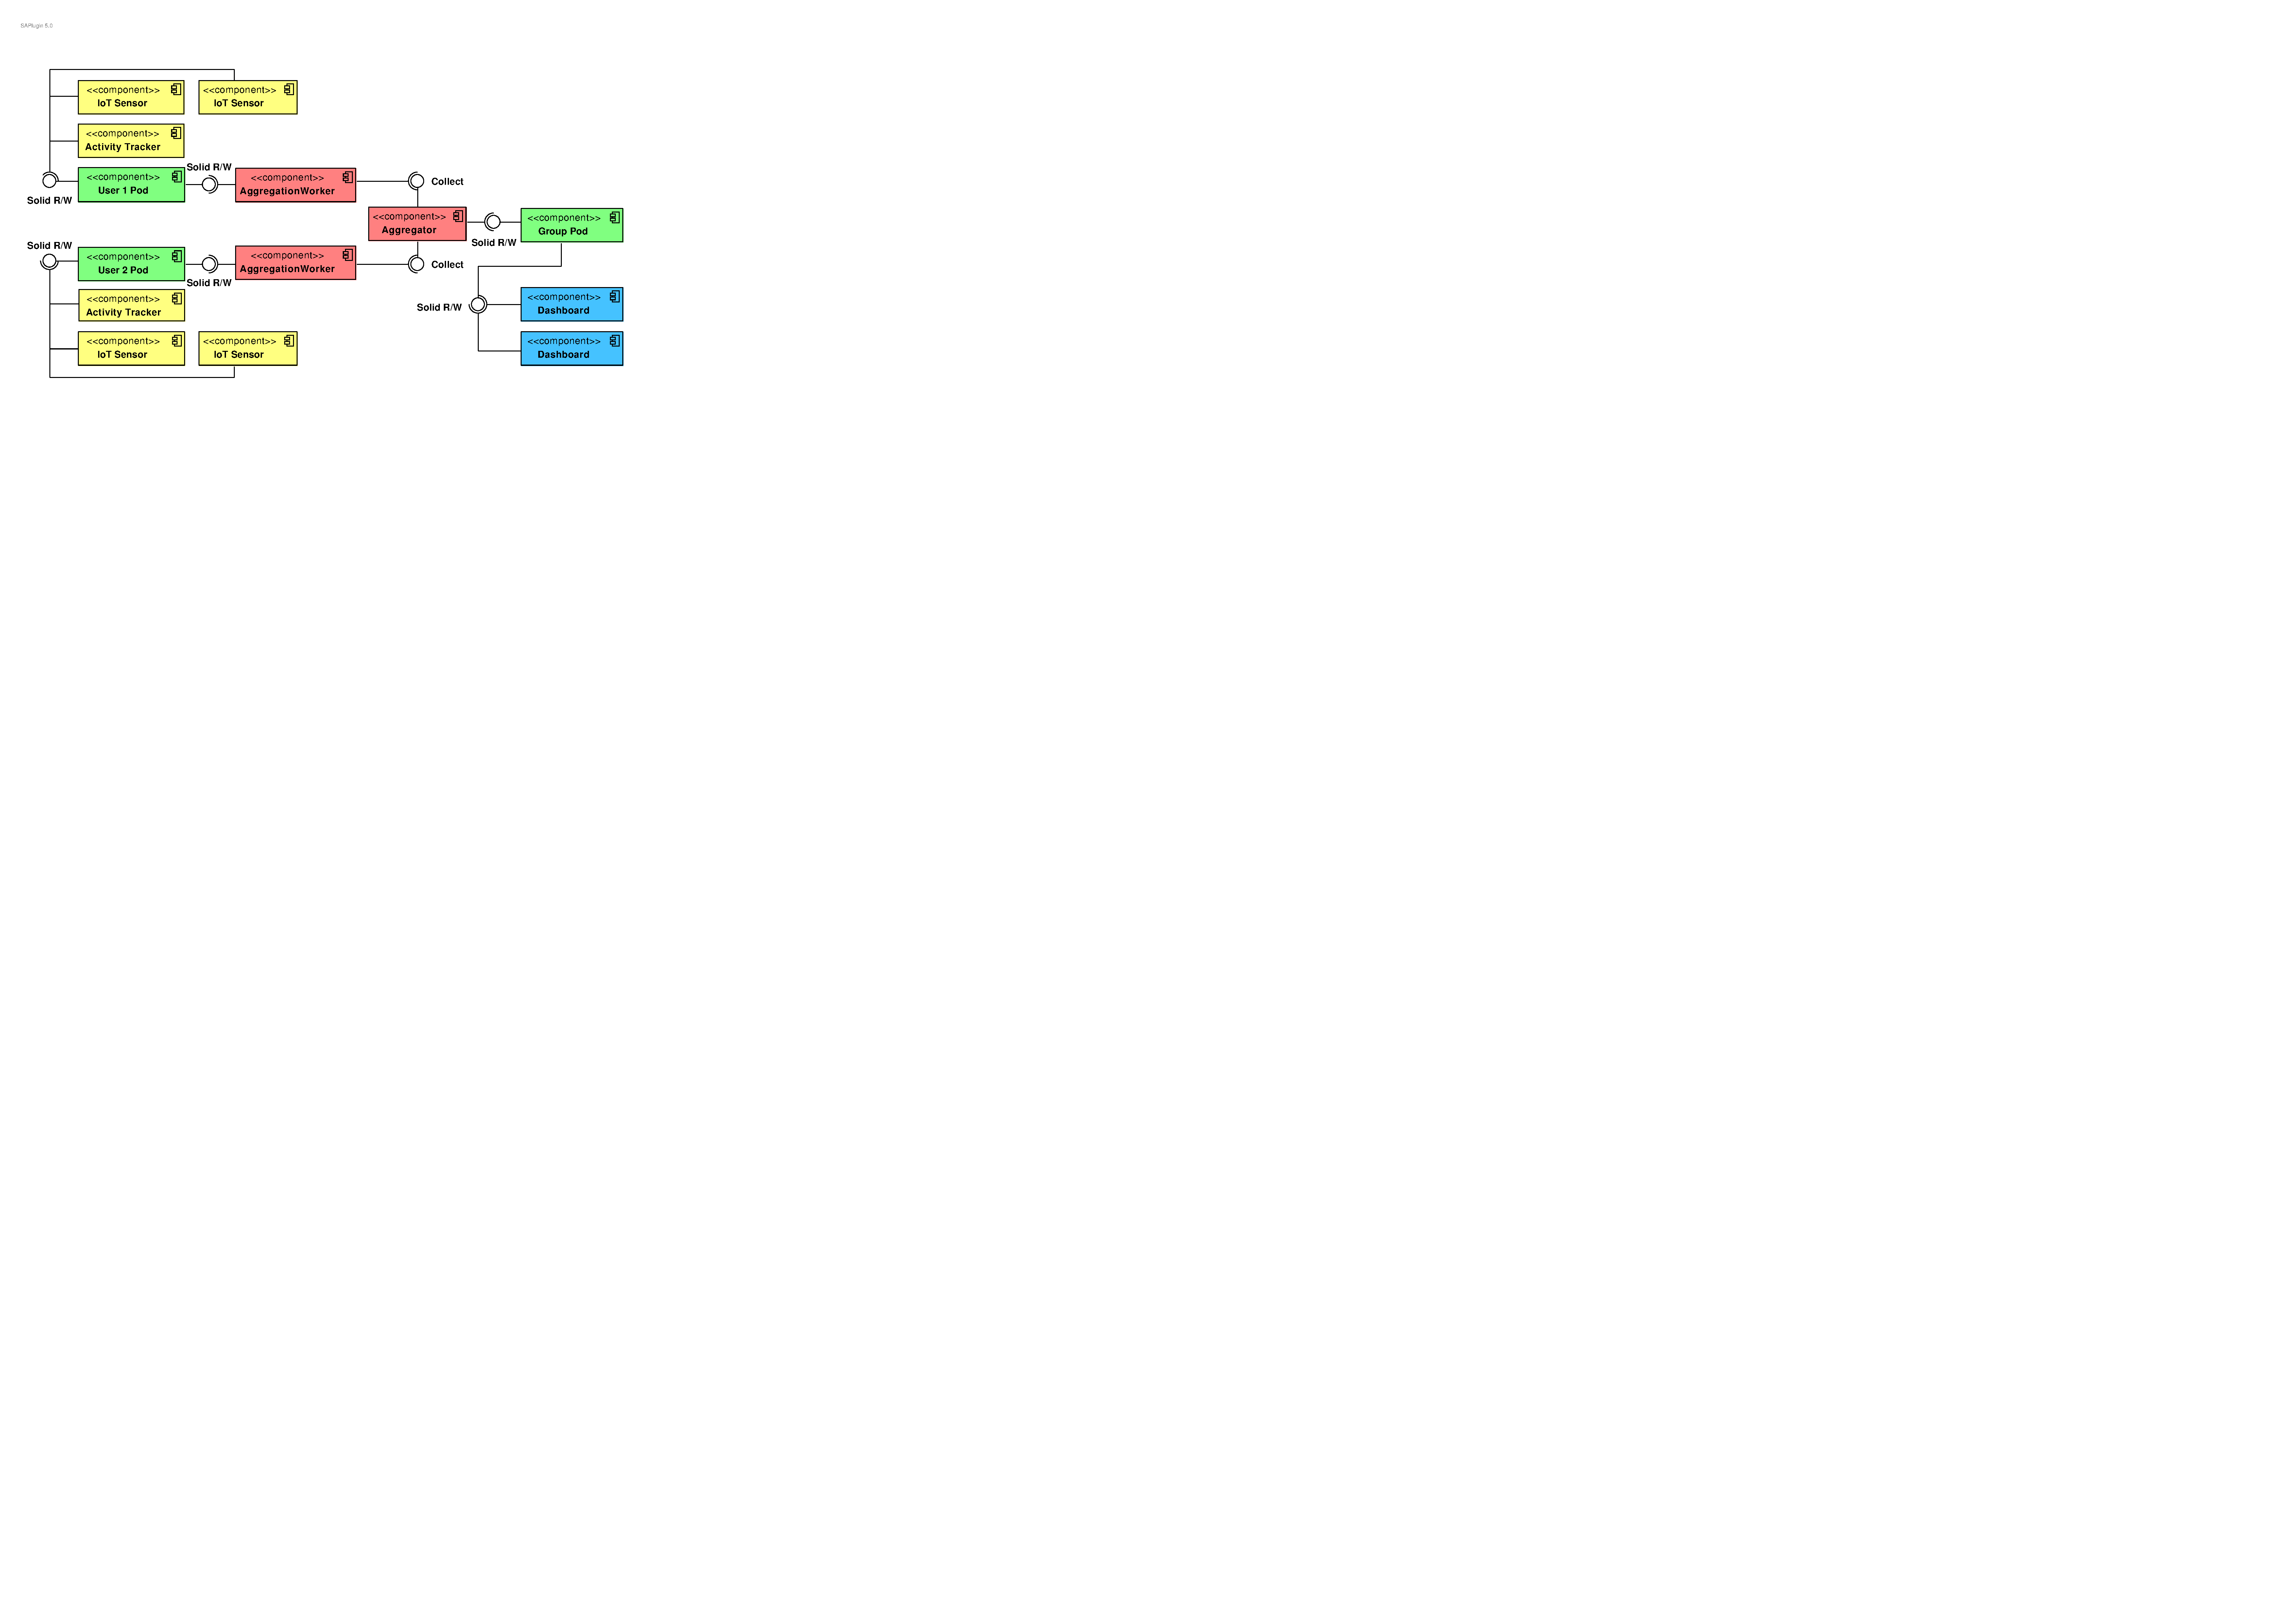
\includegraphics[width=1.0\textwidth]{images/architecture/Reference-Architecture-Aggregator.pdf}
    \caption{Reference architecture for data aggregation in Solid}
    \label{fig:reference-architecture}
\end{figure}

\noindent This reference architecture demonstrates a number of challenges that make aggregation insecure, unscalable or privacy-invasive. Concretely, the following issues are remarked.

\begin{enumerate}
    \item IoT Sensors and Activity Trackers are embedded devices that very regularly write data to a Solid Pod. As these are resource-constrained devices, this must be very efficient. As section \ref{sec:dpop} explains, the currently used mechanism uses public key cryptography, which is very computationally intensive.
    \item The aggregator component (illustrated in red on the figure) reads directly from the user's Pod. Privacy-wise, this is unsafe and unnecessary. Some method of restricting the data exposed to the aggregator must be devised.
    \item The aggregator component can consist of multiple worker nodes in different networks. Similarly, services can require data from a Solid Pod but also depend on other services that also need access to this data. This is currently not supported in Solid, and existing flows (such as OAuth On-Behalf-Of) impose bottlenecks on the token endpoint. \item Group Pods holding data of users from different Pod providers are not supported as of yet. This comes with challenges in the authentication domain.
\end{enumerate}

Problems (1), (3) and (4) are handled in chapter \ref{cha:decentralized-delegation}, while problem (2) is the topic of chapter \ref{cha:privacy-filters}.
